\documentclass[border=10pt]{standalone}
\usepackage{amsmath}
\usepackage{tikz}
\usetikzlibrary{arrows.meta, fit, backgrounds, positioning, calc}

\definecolor{inputcol}{HTML}{4FC3F7}    % light blue — inputs
\definecolor{hiddencol}{HTML}{AB47BC}   % purple — hidden/processing layers
\definecolor{outputcol}{HTML}{66BB6A}   % green — outputs
\definecolor{attncol}{HTML}{FFA726}     % orange — attention/special

\begin{document}
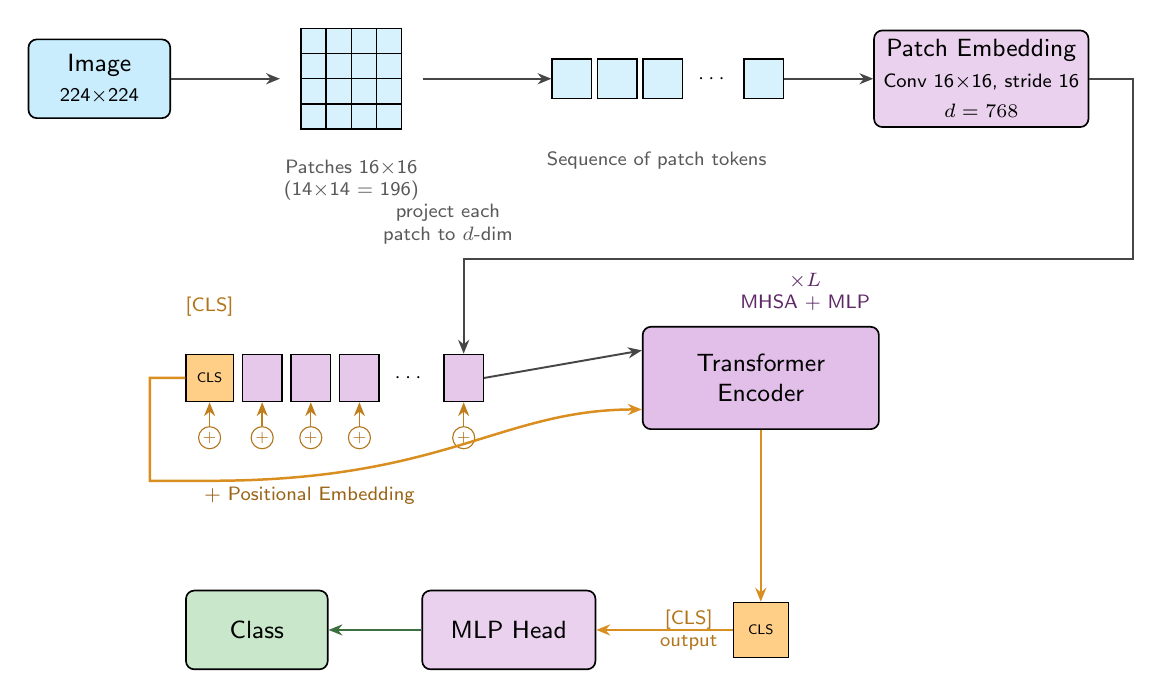
\begin{tikzpicture}[
  layer/.style={
    draw, rounded corners=3pt, minimum width=2.4cm, minimum height=1.0cm,
    font=\sffamily\small, align=center, line width=0.6pt
  },
  tok/.style={
    draw, minimum width=0.5cm, minimum height=0.5cm,
    font=\sffamily\scriptsize, align=center, line width=0.5pt
  },
  annot/.style={font=\sffamily\scriptsize, text=gray!70!black, align=center},
  conn/.style={-{Stealth[length=5pt, width=4pt]}, line width=0.7pt},
  data/.style={conn, gray!55!black},
  cls/.style={conn, attncol!85!black, line width=0.9pt}
]

% ============ ROW 1 (left -> right) ============

% 1. Input image
\node[layer, fill=inputcol!30, minimum width=1.8cm] (img) at (0,0)
  {Image\\\scriptsize 224$\times$224};

% 2. Patchify — 4x4 grid
\node[draw=none, minimum width=1.8cm, minimum height=1.0cm] (patchanchor) at (3.2,0) {};
\foreach \r in {0,1,2,3}{
  \foreach \c in {0,1,2,3}{
    \node[tok, fill=inputcol!22, minimum width=0.32cm, minimum height=0.32cm,
      font=\sffamily\tiny]
      at ($(patchanchor)+(-0.48,0.48)+(0.32*\c,-0.32*\r)$) {};
  }
}
\node[annot, below=0.55cm of patchanchor, yshift=0.15cm]
  {Patches 16$\times$16\\(14$\times$14 = 196)};

% 3. Flatten to sequence of patch tokens
\node[tok, fill=inputcol!22] (s1) at (6.0,0) {};
\node[tok, fill=inputcol!22, right=0.06cm of s1] (s2) {};
\node[tok, fill=inputcol!22, right=0.06cm of s2] (s3) {};
\node[tok, right=0.06cm of s3, draw=none, minimum width=0.3cm] (sd) {$\cdots$};
\node[tok, fill=inputcol!22, right=0.06cm of sd] (s4) {};
\node[annot, below=0.55cm of s2, xshift=0.5cm] {Sequence of patch tokens};

% 4. Patch embedding
\node[layer, fill=hiddencol!25, minimum width=2.6cm] (emb) at (11.2,0)
  {Patch Embedding\\\scriptsize Conv 16$\times$16, stride 16\\\scriptsize $d=768$};

% Row 1 connections
\draw[data] (img.east) -- (patchanchor.west);
\draw[data] (patchanchor.east) -- (s1.west);
\draw[data] (s4.east) -- (emb.west);

% turn-around elbow from emb down to row 2
\coordinate (turn) at ($(emb.east)+(0.55,0)$);

% ============ ROW 2 (right -> left) ============
\def\rowtwoy{-3.8}

% 5. CLS + positional embeddings token row
% [CLS] token (orange) at the front (leftmost in final sequence)
\node[tok, fill=attncol!55, minimum width=0.6cm, minimum height=0.6cm,
  font=\sffamily\tiny] (cls) at (1.4,\rowtwoy) {CLS};
\node[tok, fill=hiddencol!30, right=0.1cm of cls, minimum height=0.6cm] (t1) {};
\node[tok, fill=hiddencol!30, right=0.1cm of t1, minimum height=0.6cm] (t2) {};
\node[tok, fill=hiddencol!30, right=0.1cm of t2, minimum height=0.6cm] (t3) {};
\node[tok, right=0.06cm of t3, draw=none, minimum width=0.3cm] (td) {$\cdots$};
\node[tok, fill=hiddencol!30, right=0.1cm of td, minimum height=0.6cm] (t4) {};

% pos emb '+' annotation under the token row
\foreach \n in {cls,t1,t2,t3,t4}{
  \node[draw, circle, attncol!70!black, fill=white, inner sep=0pt,
    minimum size=0.28cm, font=\sffamily\tiny] (p\n) at ($(\n.south)+(0,-0.45)$) {$+$};
  \draw[conn, attncol!75!black, line width=0.5pt] (p\n) -- (\n.south);
}
\node[annot, below=0.95cm of t1, xshift=0.6cm, text=attncol!60!black]
  {$+$ Positional Embedding};
\node[annot, above=0.35cm of cls, text=attncol!70!black] {[CLS]};

% data from emb (row1) into this token row.
% route around the right side, down, and into the token row from above-right of t4
\coordinate (drop) at ($(t4.north)+(0,1.2)$);
\draw[data] (emb.east) -- (turn)
  -- (turn |- drop)
  -- (drop) -- (t4.north);
\node[annot, above=2pt of drop, anchor=south, xshift=-0.2cm] {project each\\patch to $d$-dim};

% 6. Transformer Encoder
\node[layer, fill=hiddencol!35, minimum width=3.0cm, minimum height=1.3cm] (enc)
  at (8.4,\rowtwoy) {Transformer\\Encoder};
\node[annot, above=2pt of enc.north east, anchor=south east, text=hiddencol!55!black]
  {$\times L$\\\scriptsize MHSA + MLP};

% all patch tokens -> encoder (data bus, enters upper-left of encoder)
\draw[data] (t4.east) -- ($(enc.west)+(0,0.35)$);
% cls highlighted path into encoder (routed left then below the pos-emb row)
\coordinate (clsbusy) at ($(pcls.south)+(0,-0.4)$);
\draw[cls] (cls.west) -| ($(cls.west)+(-0.45,0)$) |- (clsbusy)
  .. controls +(3.0,0) and +(-1.8,0) .. ($(enc.west)+(0,-0.4)$);

% ============ ROW 3 — output ============
\def\rowthreey{-7.0}

% 7. CLS output -> MLP Head -> Class
\node[tok, fill=attncol!55, minimum width=0.7cm, minimum height=0.7cm,
  font=\sffamily\tiny] (clsout) at (8.4,\rowthreey) {CLS};
\node[annot, left=2pt of clsout, text=attncol!70!black, anchor=east]
  {[CLS]\\output};

\node[layer, fill=hiddencol!25, minimum width=2.2cm] (mlp) at (5.2,\rowthreey)
  {MLP Head};
\node[layer, fill=outputcol!35, minimum width=1.8cm] (class) at (2.0,\rowthreey)
  {Class};

% encoder output: only the CLS token output is tapped
\draw[cls] (enc.south) -- (clsout.north);
\draw[cls] (clsout.west) -- (mlp.east);
\draw[conn, outputcol!60!black, line width=0.8pt] (mlp.west) -- (class.east);

\end{tikzpicture}
\end{document}
